\documentclass[english]{article}
\usepackage[T1]{fontenc}
\usepackage[utf8]{inputenc}
\usepackage{babel}
\usepackage[unicode=true,pdfusetitle,
 bookmarks=true,bookmarksnumbered=false,bookmarksopen=false,
 breaklinks=true,pdfborder={0 0 1},backref=false,colorlinks=false]
 {hyperref}
\usepackage{tabularx}
\usepackage{graphicx}
\graphicspath{{images/}}
\usepackage{svg}
\usepackage{float}
\usepackage{titling}
\renewcommand{\arraystretch}{1.4}
\newcommand{\code}[1]{\texttt{#1}}
\usepackage{listings}
\usepackage{color}
\definecolor{javared}{rgb}{0.6,0,0} % for strings
\definecolor{javagreen}{rgb}{0.25,0.5,0.35} % comments
\definecolor{javapurple}{rgb}{0.5,0,0.35} % keywords
\definecolor{javadocblue}{rgb}{0.25,0.35,0.75} % javadoc

\lstset{language=Java,
	basicstyle=\ttfamily\small,
	xleftmargin=-2cm,
	keywordstyle=\color{javapurple}\bfseries,
	stringstyle=\color{javared},
	commentstyle=\color{javagreen},
	morecomment=[s][\color{javadocblue}]{/**}{*/},
	numbers=left,
	numberstyle=\tiny\color{black},
	stepnumber=1,
	numbersep=10pt,
	tabsize=4,
	showspaces=false,
	showstringspaces=false,
	linewidth=16cm,
	breaklines=true
	}

\pretitle{%
	\begin{center}
		\LARGE
		
\includegraphics[width=250pt]{../other/Logo_blu.png}\\[\bigskipamount]~\\[\bigskipamount]
	}
\posttitle{\end{center}}

\begin{document}

\title{Politecnico di Milano\\
 A.A. 2016–2017 \\
Software Engineering 2: “PowerEnJoy” \\
\emph{Design Document}}

\author{Pietro Ferretti, Nicole Gervasoni, Danilo Labanca}
\date{December 11, 2016}
\maketitle

\newpage

\tableofcontents{}

\newpage

\section{Introduction}

\subsection{Purpose}

\paragraph{}
The purpose of this document is to specify in a more technical way how our system is designed to be built and work. 
This document is intended for developers, designers and all interested stakeholders as a guideline for the implementation of the system.

\paragraph{}
This document will first of all illustrate the system architecture, the components that make it up and how each of its components is designed to interact with each other.

Furthermore this document will describe the behaviour of the system and the applications, from both the back-end and the front-end side.

Finally this document will describe the patterns we used to design the system and how each of them comes into play.

%% magari ridurre a due righe ^^^


\subsection{Scope}
\paragraph{}
The aim of this project is to specify in detail a new digital management software for PowerEnJoy, a car-sharing service that employs electric cars only.
%
%\paragraph{}
PowerEnjoy will offer a very valuable service to its users, letting them borrow cars to drive around the city freely, as an alternative to their own vehicles and public transport.
%Among the advantages of using PowerEnJoy we can note being able to find available cars in any place that is served by our system and having dedicated spots to park in (namely, PowerEnJoy's power grid stations). 
%Furthermore, thanks to the fact that all the cars that we provide are electrically powered, PowerEnJoy is also very environmentally friendly.

\paragraph{}
PowerEnJoy's users, after registering, will be able to reserve, unlock and drive the cars our system will provide. Users will be charged per minute until they park the car in a safe area and end the ride.
Users will be able to park their car temporarily and use it again later, or end their ride remotely.

Our system will incentivize virtuous behaviour by offering several discounts if certain conditions are met (like charging a car at a power grid station).


\newpage
\subsection{Definitions, Acronyms, Abbreviations}

% vanno tolte le definizioni che non vengono usate in questo documento
% e aggiunte quelle in più

\subsubsection{Definitions}

\begin{itemize}
\item{\textit{Guest}: a person that is not registered to the system.}
\item{\textit{User}: a person that is registered to the system. Users can log in to the system with their email or username and their password. Their first name, last name, date of birth, driving license ID are stored in the database.}
\item{\textit{Safe area}: a location where the user can park and leave the car. Users can end their ride and park temporarily only in these locations. The set of safe areas is predefined by the system.}
\item{\textit{Power grid station}: a place where cars can be parked and plugged in. While a car is plugged in a power grid station its battery will be recharged. Power grid stations are by definition safe areas.}
\item{\textit{Available car}: a car that is currently not being used by any user, and has not been reserved either. Available cars are in good conditions (not dirty nor damaged) and don’t have dead batteries.}
\item{\textit{Reservation}:
	\begin{itemize}
		\item{the operation of making a car reserved for a user, i.e. giving permission to unlock and use the car only for that user, forbidding reservations by other users.}
		\item{the time period between the moment a reservation is requested and the moment the user unlocks the car, or the reservation is canceled.}
	\end{itemize}
}
\item{\textit{Ride}: the time period from the moment a reserved car is unlocked to the moment the user notifies that he wants to stop using the car and closes all the doors. A ride doesn’t stop when a car is temporarily parked, but continues until the user chooses to leave the car definitely.}
\item{\textit{Possession}: users that have reserved and unlocked a car are said to have possession of the car. While a user has possession of a car they are the only person that can drive it, lock or unlock it, and no other person can take possession of it until the user frees it. Users lose possession of a car when their ride ends.}
\item{\textit{Temporary parking}: the act of parking a car in a safe area and, after notifying the system, locking it and leaving it for a finite amount of time. The user that does this retains the right to use the car and can unlock it later to use it again.}
\item{\textit{Bill}: a record of the money owed by the user at the end of a ride.}
\item{\textit{Outstanding bill}: a bill that hasn’t been paid yet. }
\item{\textit{Suspended user}: a user that cannot reserve or use cars. Usually users are suspended because they have outstanding bills.}
\item{\textit{Payment method}: a way to transfer money from the user to the system. Our system will only accept credit cards and online accounts like Paypal.}
\item{\textit{Payment API}: an interface to carry out money transactions, offered by the external provider associated to the payment method used (e.g. a bank).}
\item{\textit{CAN bus}: a vehicle bus standard designed to allow micro controllers and devices to communicate with each other.}
\end{itemize}

\subsubsection{Acronyms}
\begin{itemize}
\item{\textbf{DD}: Design Document}
\item{\textbf{RASD}: Requirements Analysis and Specification Document}
\item{\textbf{DB}: Database}
\item{\textbf{CVV}: Card Verification Value}
\item{\textbf{DOB}: Date of birth}
\item{\textbf{PGS}: Power Grid Station}
\item{\textbf{GPS}: Global Positioning System}
\item{\textbf{CAN bus}: Controller Area Network bus}
\end{itemize}

\subsubsection{Abbreviations}
\begin{itemize}
\item{\textbf{[Gx]}: Goal}
\item{\textbf{[RE.x]}: Functional Requirement}
\item{\textbf{[UC.x]}: Use Case}
\end{itemize}

\subsection{Reference Documents}

\begin{itemize}
	\item{IEEE Std. 1016-2009, “IEEE Standard for Information Technology -- Systems Design -- Software Design Descriptions”}
	\item{ISO/IEC/IEEE Std. 42010:2011, “Systems and software engineering -- Architecture Description”}
	\item{Specification document: “Assignments AA 2016-2017.pdf”}
\end{itemize}

\newpage{}

\subsection{Document Structure}

This document is structured as follows:
\begin{itemize}
\item{\textbf{Section 1 -- Introduction} }
\item{\textbf{Section 2 -- Architectural Design}
	\begin{itemize}
		\item{\textbf{Overview:} this section shows a high-level view of our system's architecture.}
		\item{\textbf{Component View:} this section contains a more detailed and in-depth analysis of the components that comprise the architecture, and how they interact with each other.}
		\item{\textbf{Deployment View:} this section shows how the architecture components will be deployed on physical machines.}
		\item{\textbf{Runtime View:} in this section we use sequence diagrams to show the flow of events for the most significant functionalities of the application.}
		\item{\textbf{Component Interfaces:} the interfaces between the various components are presented in this section.}
		\item{\textbf{Selected Architectural Styles and Patterns:} this section explains the architectural choices taken and the patterns followed during the creation of the application.}
	\end{itemize}}
\item{\textbf{Section 3 -- Algorithm Design:} this section proposes algorithms to realize some of the most important functionalities. A quick complexity analysis is also included.}
\item{\textbf{Section 4 -- User Interface Design:} this section formalizes with more details the user interfaces shown and described in the RASD, using UX and BCE diagrams.}
\item{\textbf{Section 5 -- Requirements Traceability:} this section aims to explain how the goals identified in the RASD are linked to the design and architecture elements described in this document.}
\item{\textbf{Effort Spent} }
\item{\textbf{References} }
\item{\textbf{Revisions} }
\end{itemize}

\newpage

\section{Architectural Design}

\subsection{Overview}

To satisfy our requirements we rely on a primarily client-server architecture. We identified three main types of clients: the mobile/web application, the vehicle application, and the embedded systems that keep track of the sensors in cars and power grid stations.

\paragraph{}
We decided to adopt a web-based framework (e.g. PhoneGap) to develop the mobile application, so that it would work very similarly to the web one, without needing to design a different interface.

The mobile/web application will first request the necessary web pages and scripts from the dedicated Web Application Server, then the scripts will collect data from the central server via a REST API as needed.

\paragraph{}
The vehicle application is not web based and will contact only the central server to get data and send requests.

\paragraph{}
The vehicle and the power grid stations will periodically send updates to the central servers. Cars must also be  listening for commands from the servers.


\begin{figure}[H]
	\centering
	\makebox[\textwidth][c]{
		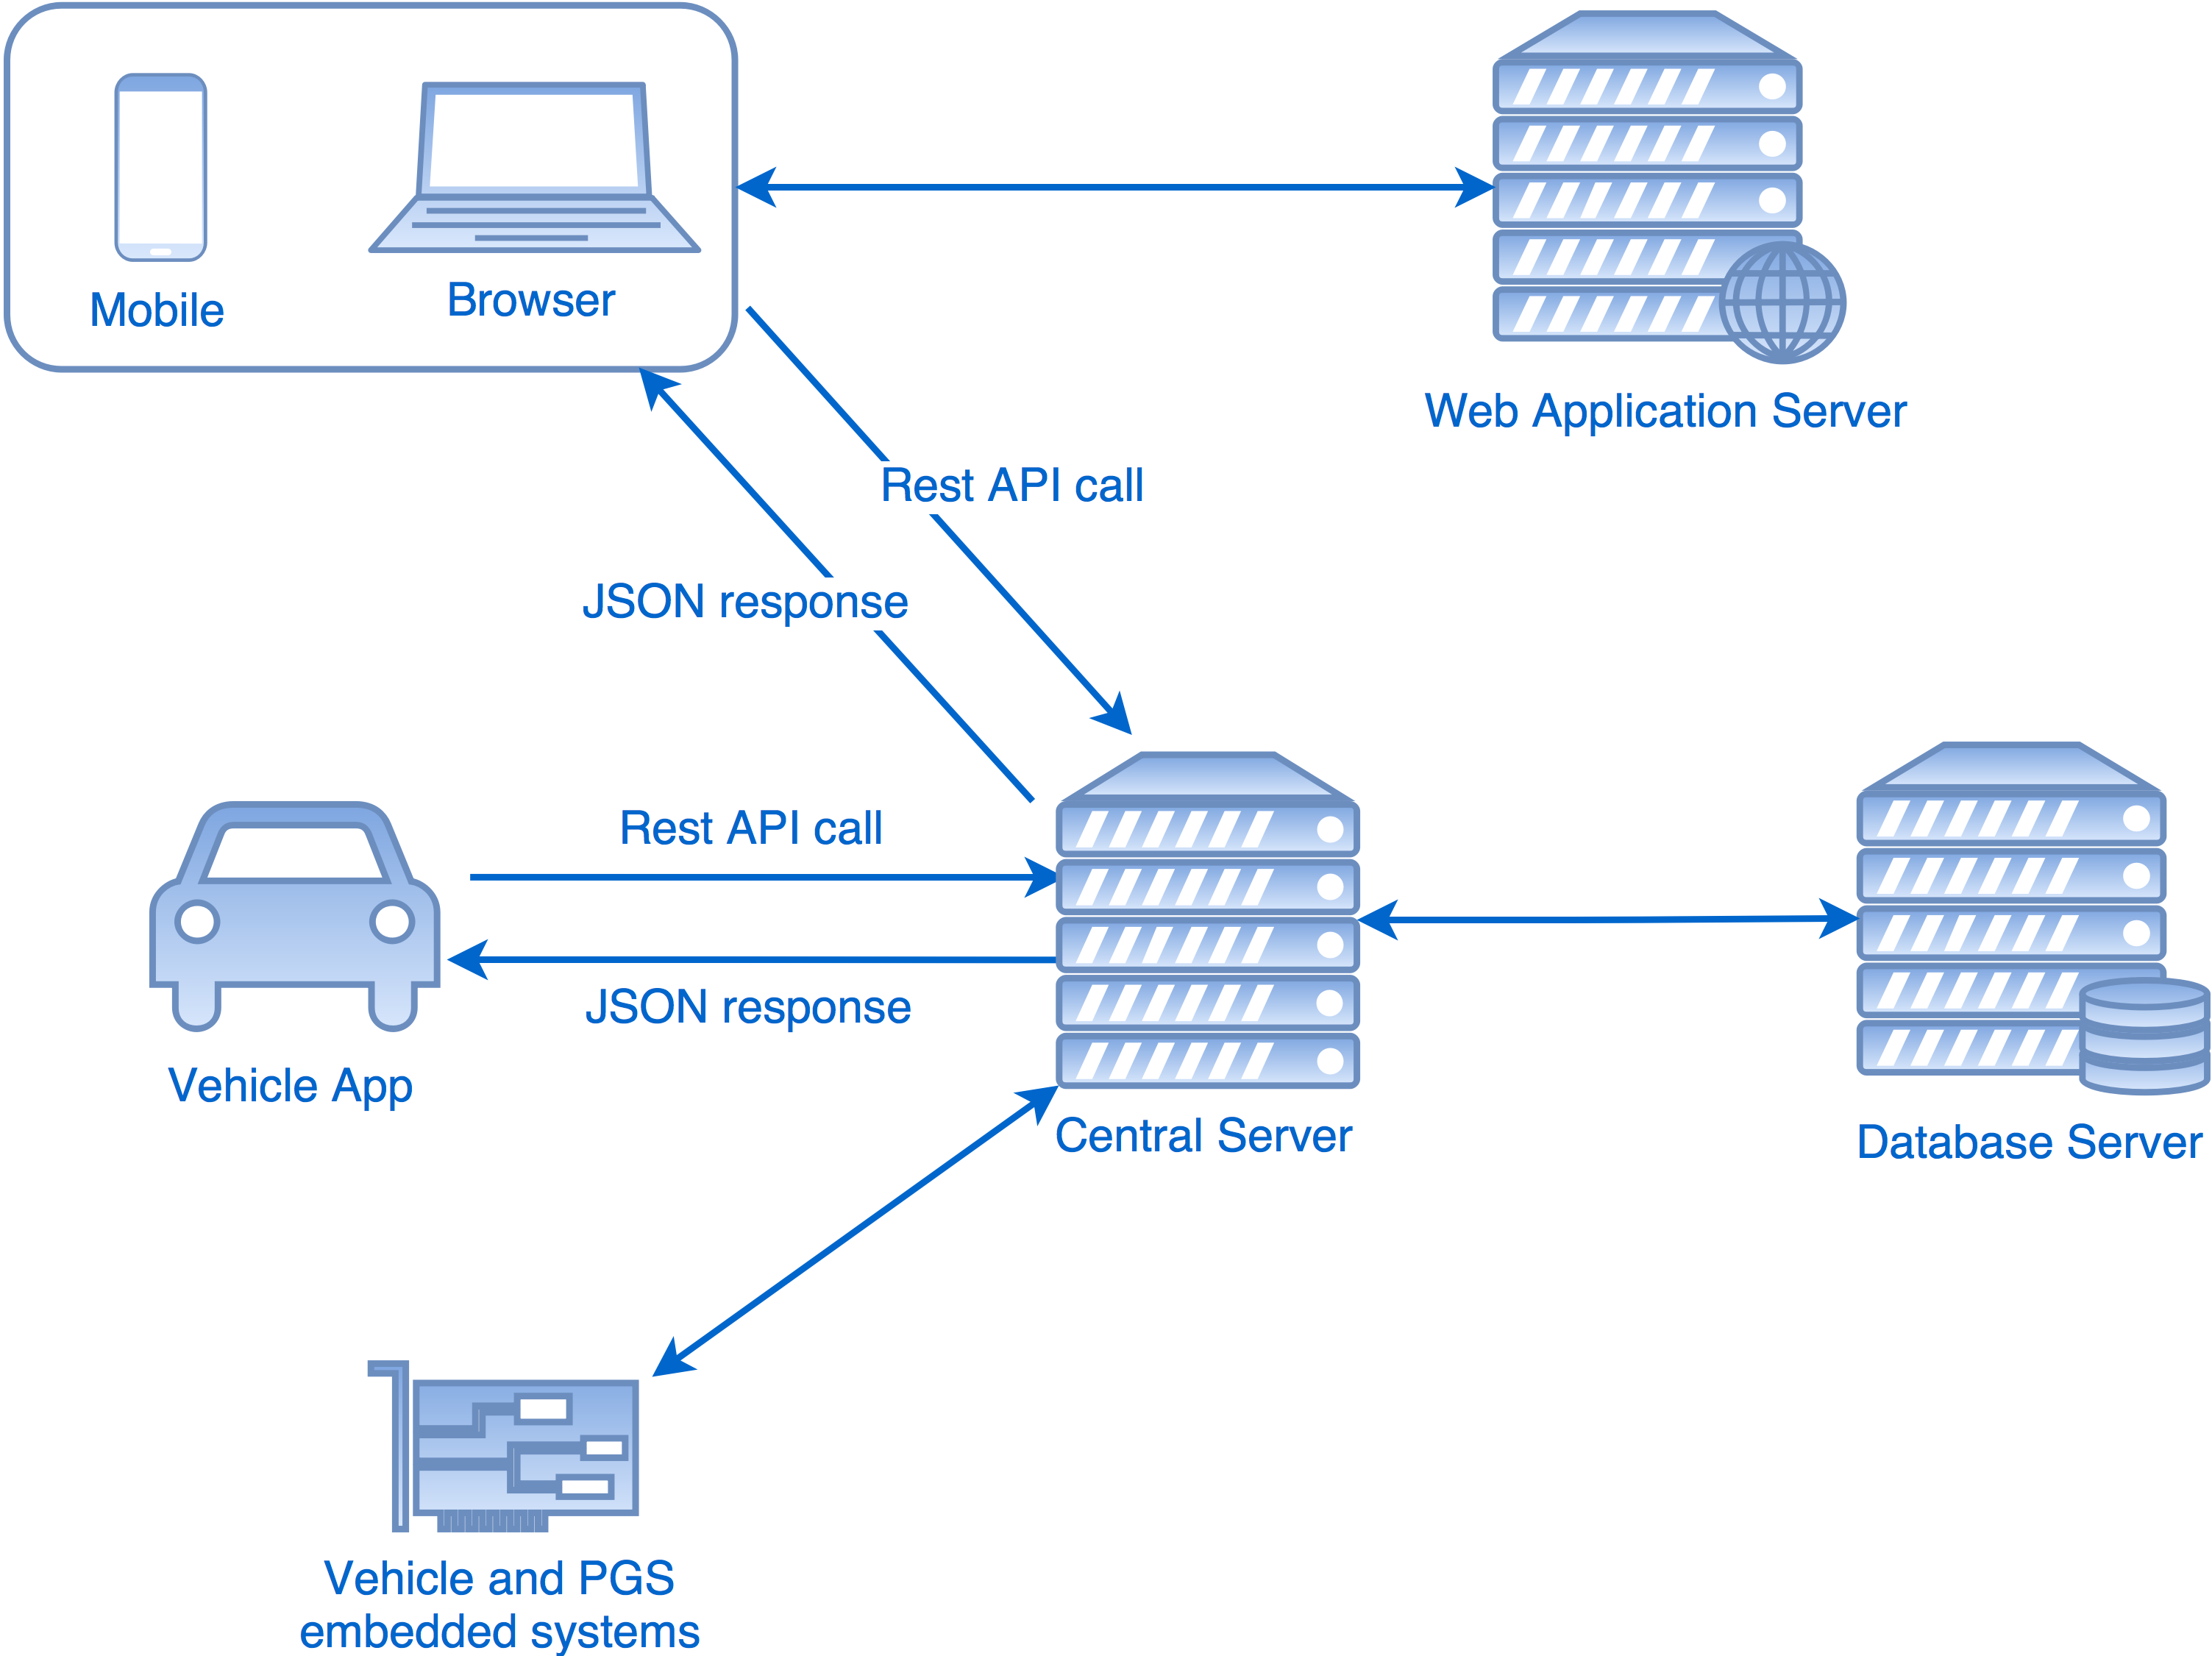
\includegraphics[width=350pt]{architecture_overview.png}
	}
	\caption{Architecture Overview}
	\label{architectureoverview}
\end{figure}


\subsection{Component View}

\begin{figure}[H]
	\centering
	\makebox[\textwidth][c]{
		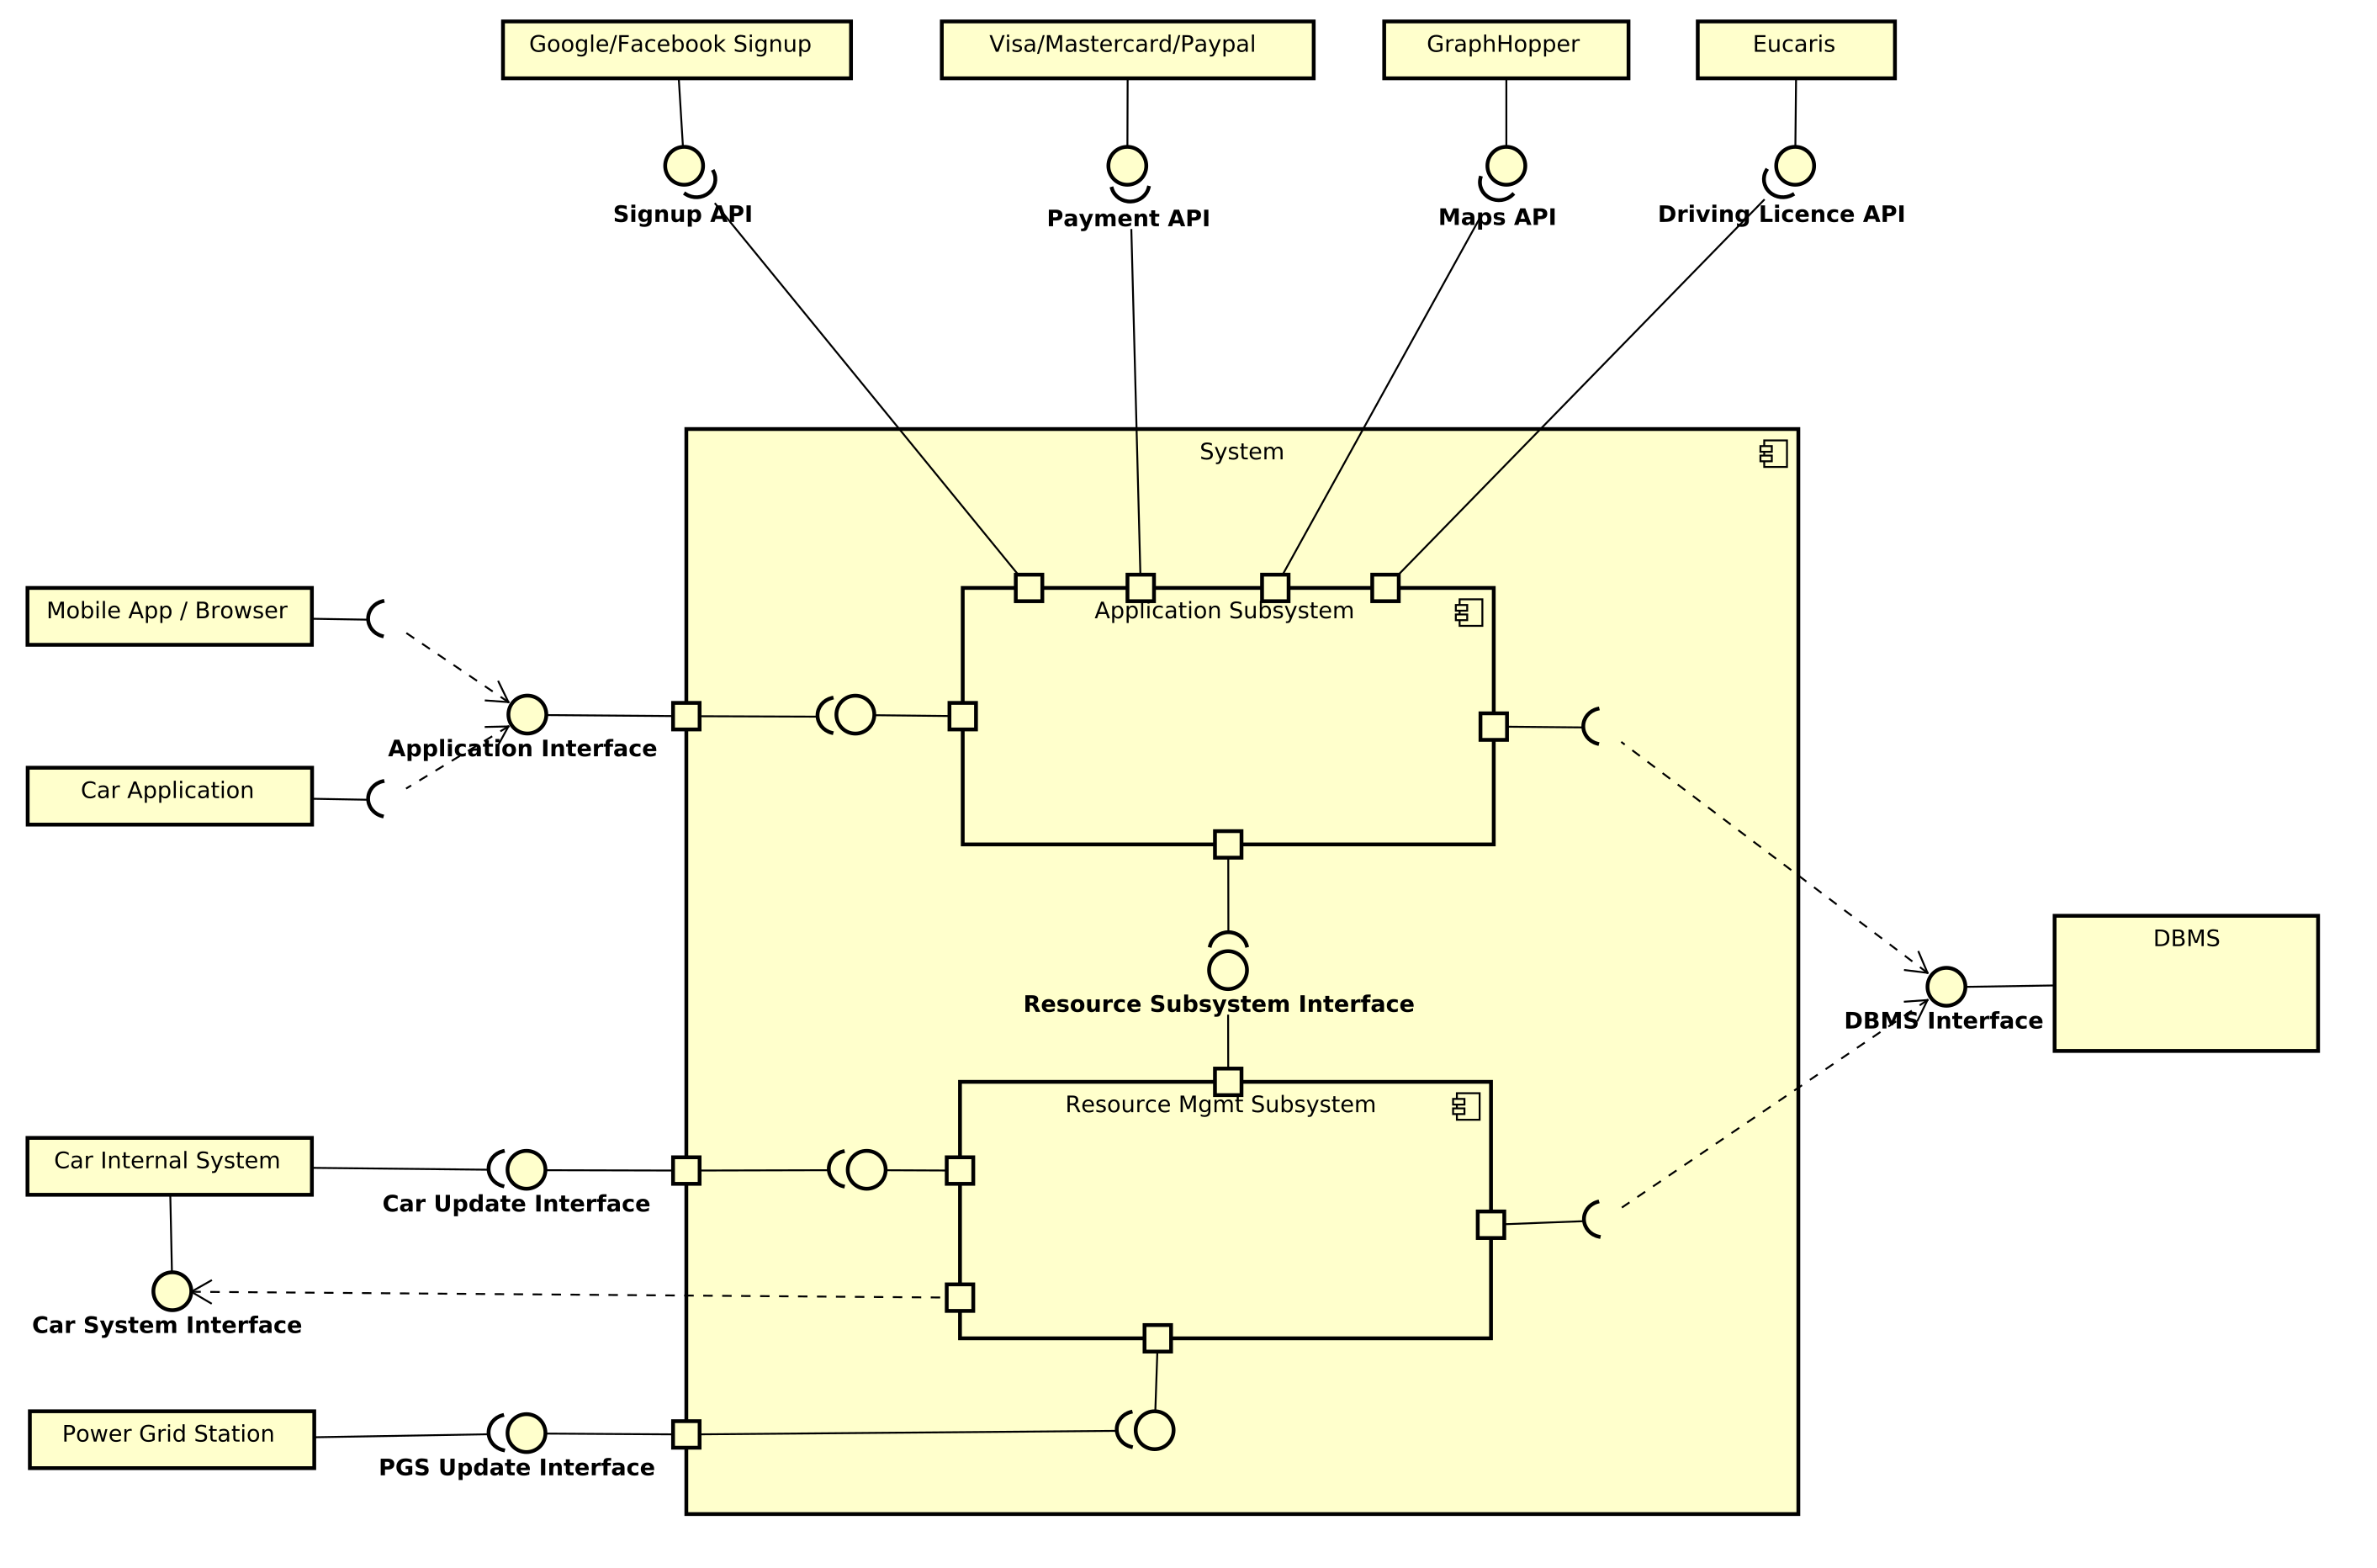
\includegraphics[width=450pt]{comp_1b.png}
	}
	\caption{Component Diagram Overview}
	\label{componentdiagram1}
\end{figure}
\begin{figure}[H]
	\centering
	\makebox[\textwidth][c]{
		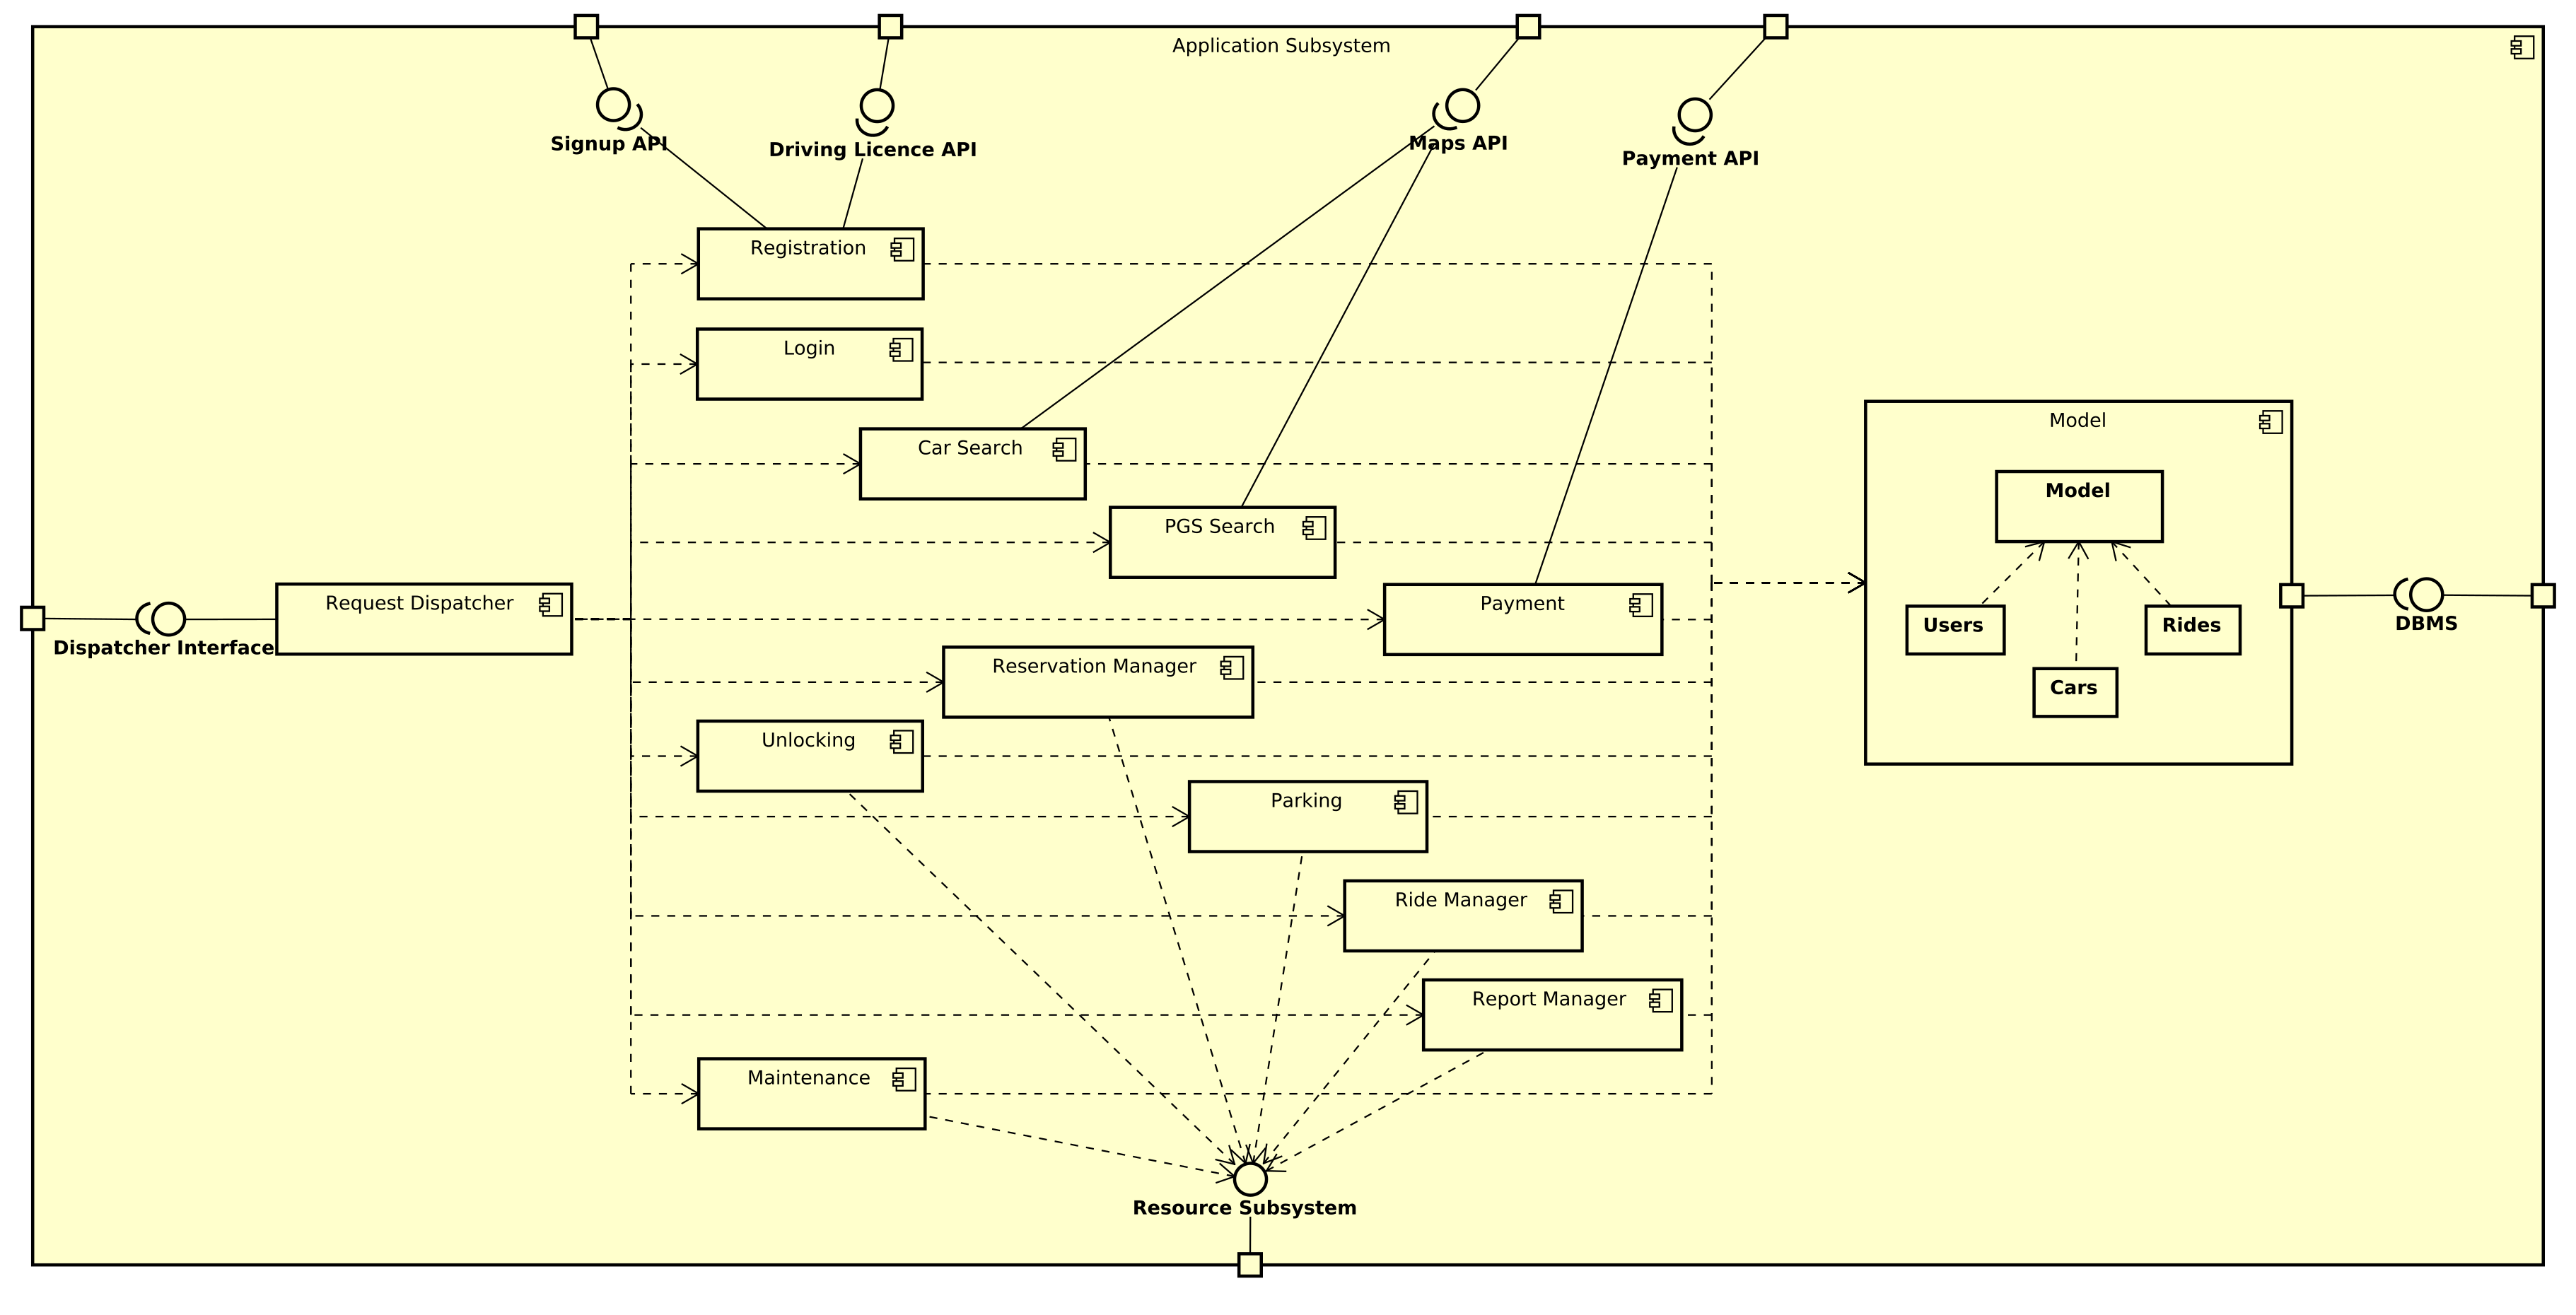
\includegraphics[width=450pt]{comp_2b.png}
	}
	\caption{Component Diagram for the Application Subsystem}
	\label{componentdiagram2}
\end{figure}
\begin{figure}[H]
	\centering
	\makebox[\textwidth][c]{
		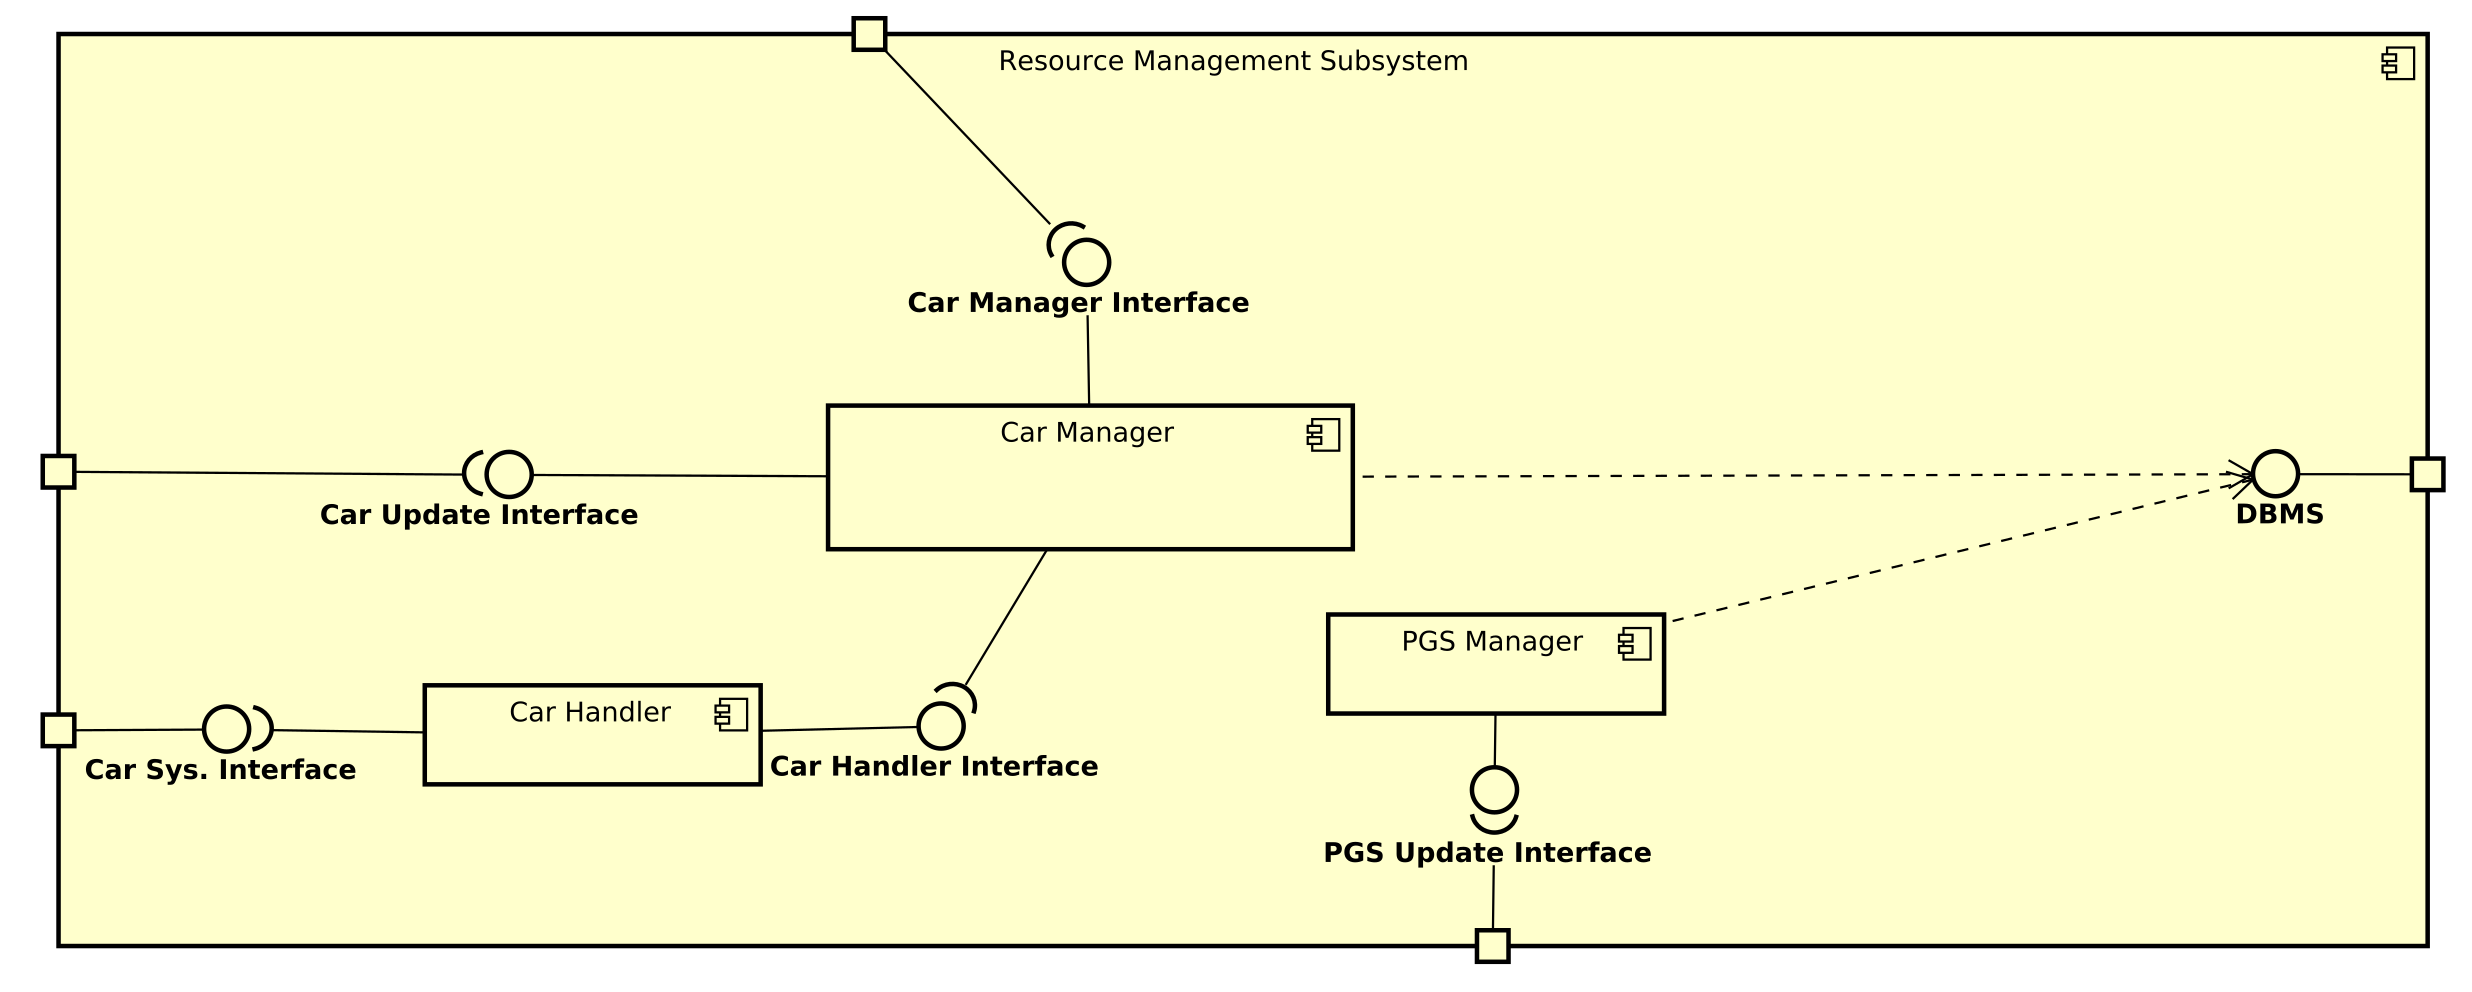
\includegraphics[width=400pt]{comp_3b.png}
	}
	\caption{Component Diagram for the Resource Management Subsystem}
	\label{componentdiagram3}
\end{figure}

\newpage
The system offers many different interfaces, each for a different role:
\begin{itemize}
	\item{an Application Interface for the mobile, web and the car applications to connect;}
	\item{a Car Update Interface through which the cars can send updates about their state to the system;} 
	\item{a Maintenance Interface to let the people in charge of this mark a car as available when it is repaired or recharged;}
	\item{a PGS Update Interface for the power grid stations' systems to send updates about the state of the plugs.}
\end{itemize}

Furthermore, the car itself has an interface to receive commands from the main system (like unlocking the doors).

The main system can run queries on the DBMS through a dedicated interface.

The external APIs used by the system are also depicted.

\paragraph{}
The main system is divided into two macro-components: the Application Subsystem and the Resource Management Subsystem.
The first handles all the operations related to the user applications and interfaces, while the second takes care of keeping track of all the automatic updates from the sensors in the cars and the charging stations.

The separation lets us manage the two families of functionalities in a more flexible way, by decoupling them. For example the Resource Subsystem could be considered as more critical for our system, and be run on servers that are more reliable and resistant to failure.

\paragraph{}
On the Application Subsystem the Request Dispatcher collects all types of requests (searches, reservations...) and redirects them to the specific components. 
The Application Subsystem can send requests to the Resource Subsystem, for example to unlock a car.
The Model is a representation of the data contained in the DBMS in a certain moment. It lets us cache information instead of having to query the database for every operation.

\paragraph{}
On the Resource Management Subsystem the Car Manager is the main component, and is in charge of handling everything that involves cars. The Car Handler keeps a list of all available cars and acts as an interface when a command needs to be sent to a car.
The PGS Manager's task is to collect updates from the power grid stations about the plugs' availability and update the database accordingly.

\newpage
\subsection{Deployment View}

\paragraph{}

\begin{figure}[H]
	\centering
	\makebox[\textwidth][c]{
		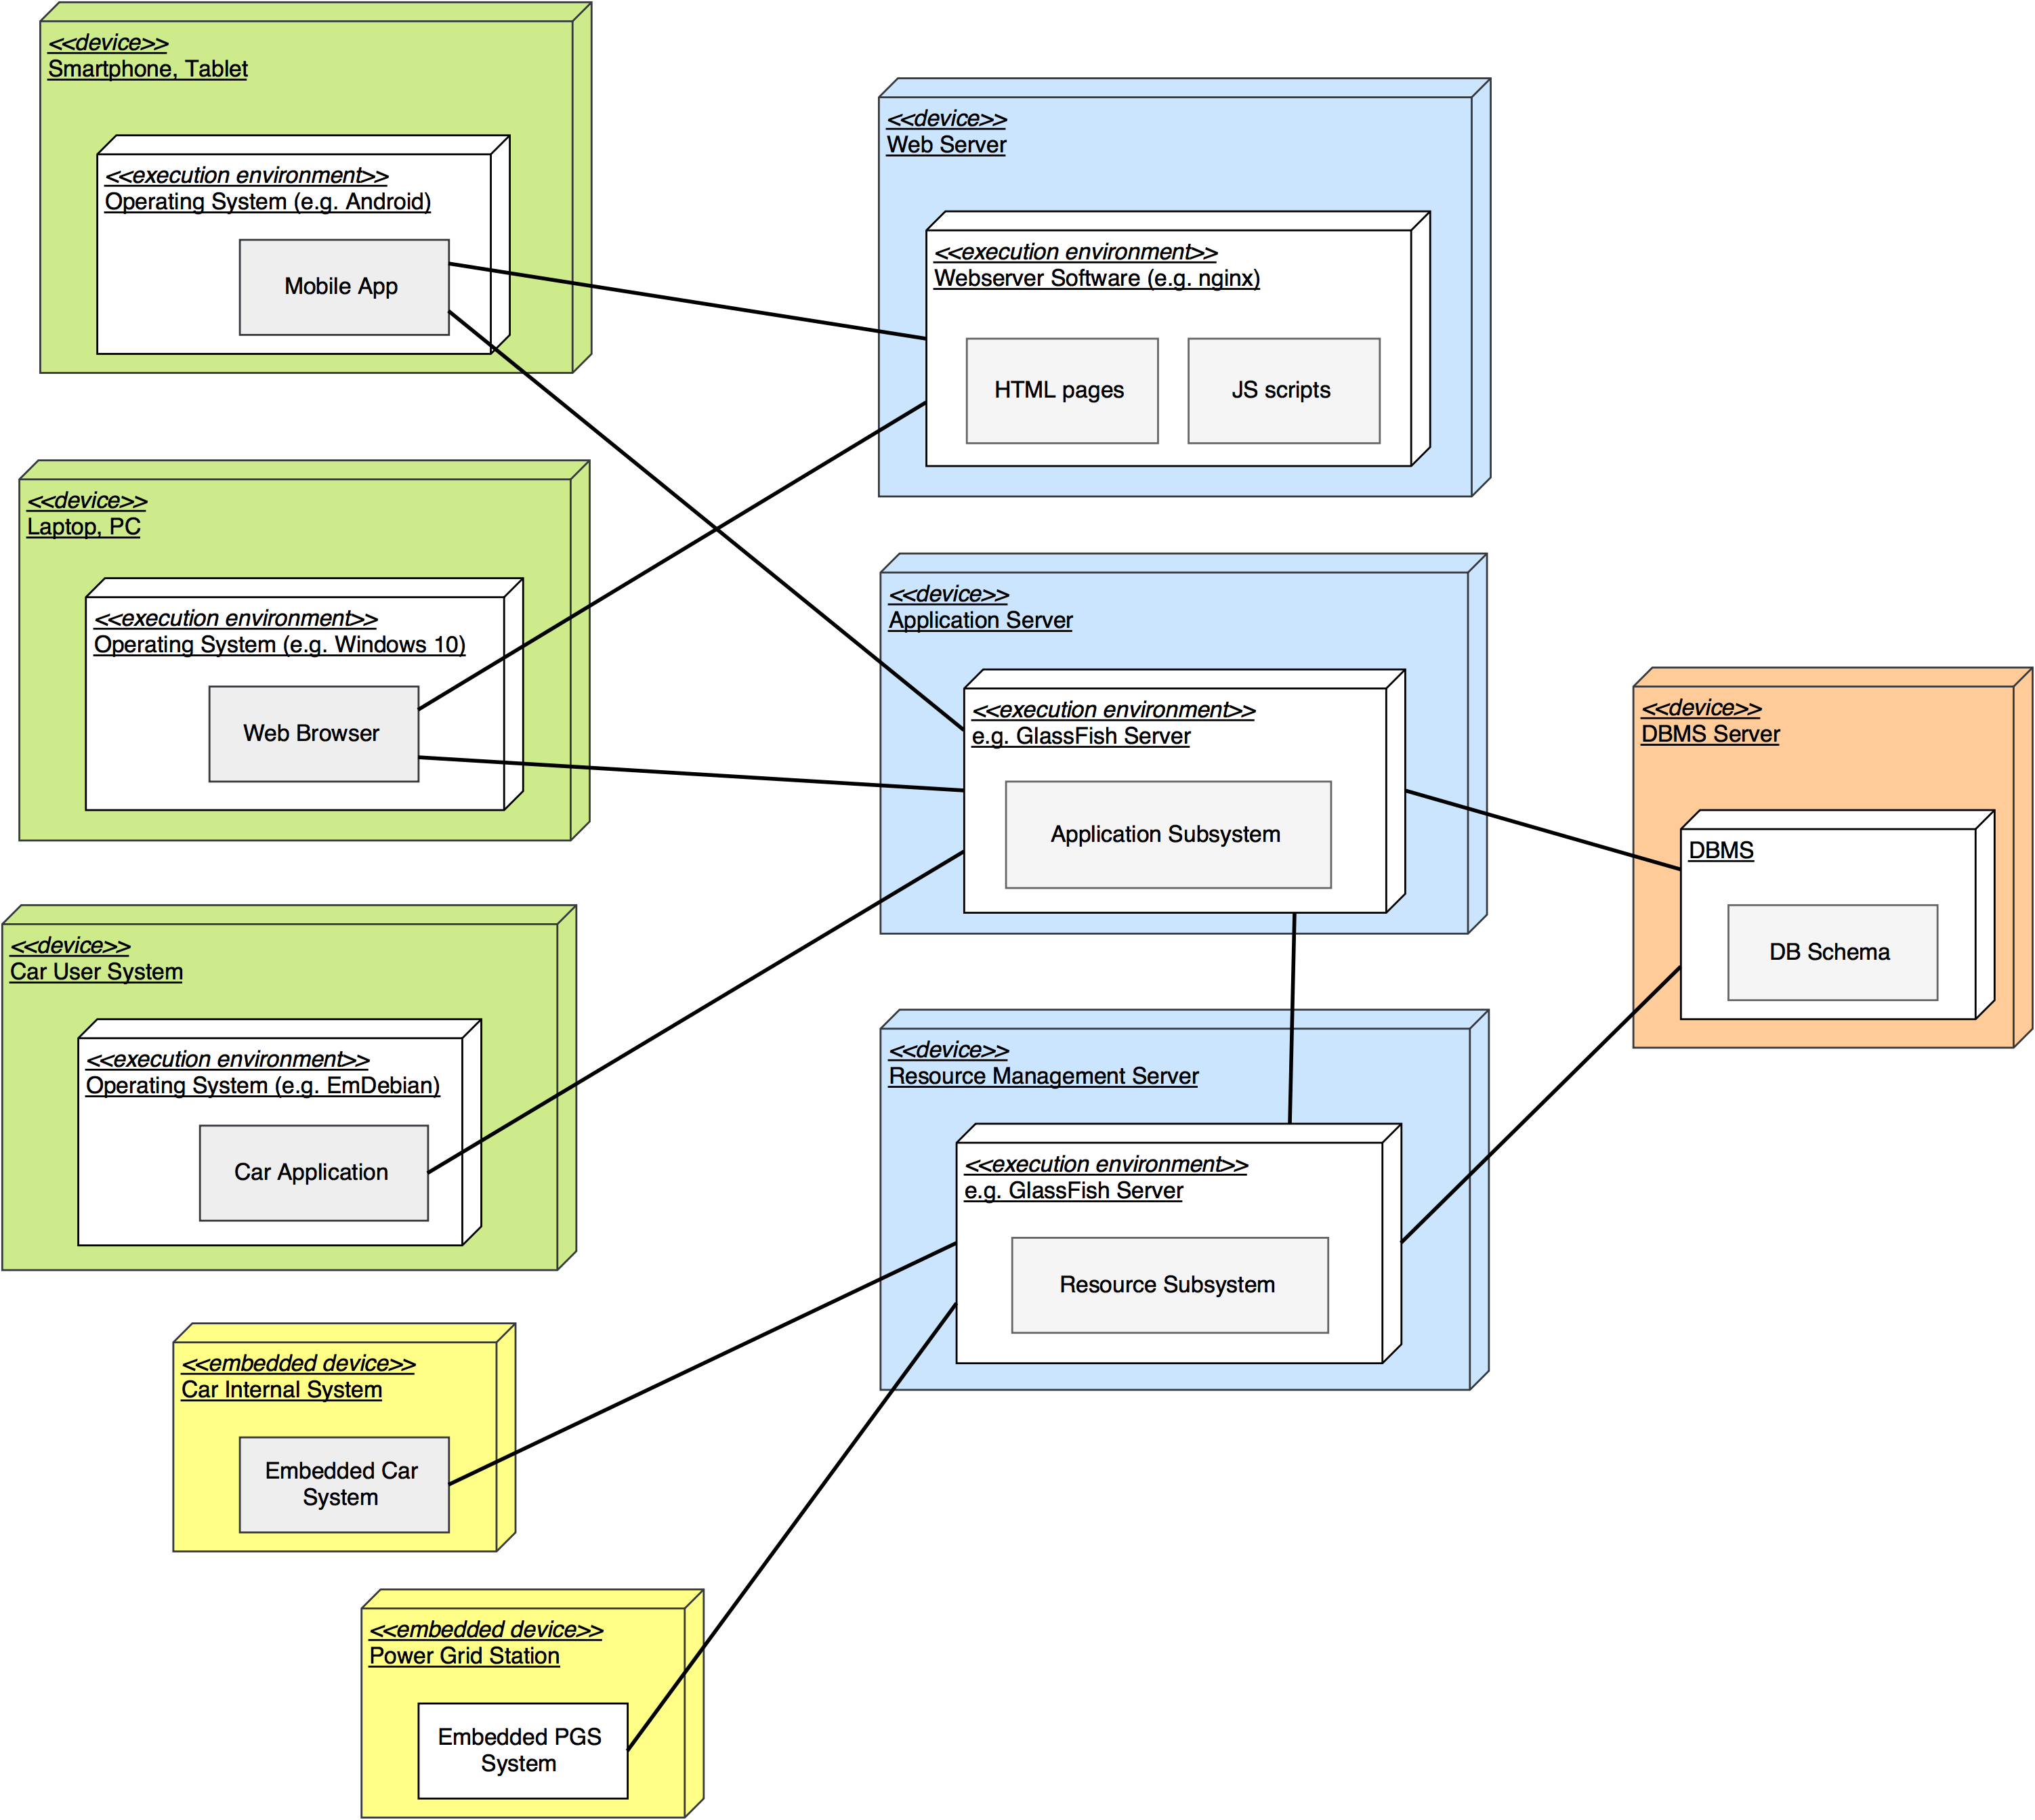
\includegraphics[width=460pt]{deployment_diagram.png}
	}
	\caption{Deployment Diagram}
	\label{deploymentdiagram}
\end{figure}

\paragraph{}
The system will be deployed on three tiers: Client, Business Logic and Data, identified by different colors. The green elements are user interfaces, the yellow ones are embedded systems.

\paragraph{}
Web and mobile application will both connect initially to the web server to obtain the markup and scripts needed to display the requested pages, then the scripts will collect the actual data from the Application Server's API.
(NB: web and mobile application are both based on web technologies and are designed to work in the same way, with a framework like PhoneGap)

The car application is "thicker" and not web based. It doesn't need to request the web pages from the Web Server, but will just get data from the Application Server.

\paragraph{}
The Resource Management Server manages updates sent by cars (about their GPS position, engine status and everything else) and power grid stations (about plugs availability).
Every car listens for incoming commands from the Resource Server; the Application Server has a a direct connection to the Resource Server to send commands directly to the cars.

\paragraph{}
The Application Server and the Resource Management Server are both connected to the DBMS to get data or update the database.

\newpage
\subsection{Runtime View}

% sequence diagrams
\subsubsection{Registration}
\begin{figure}[H]
	\centering
	\makebox[\textwidth][c]{
		\def\svgwidth{450pt}
		\input{images/registration.pdf_tex}
	}
	\caption{Registration}
	\label{seq_registration}
\end{figure}

\subsubsection{Car Search}
\begin{figure}[H]
	\centering
	\makebox[\textwidth][c]{
		\def\svgwidth{450pt}
		\input{images/car_search.pdf_tex}
	}
	\caption{Car Search}
	\label{seq_carsearch}
\end{figure}

\subsubsection{Unlocking a car}
\begin{figure}[H]
	\centering
	\makebox[\textwidth][c]{
		\def\svgwidth{450pt}
		\input{images/car_unlock.pdf_tex}
	}
	\caption{Car Unlocking}
	\label{seq_carunlock}
\end{figure}

\subsubsection{Payment}
\begin{figure}[H]
	\centering
	\makebox[\textwidth][c]{
		\def\svgwidth{450pt}
		\input{images/payment.pdf_tex}
	}
	\caption{Payment}
	\label{seq_payment}
\end{figure}

\subsubsection{Setting a car as unavailable}
\begin{figure}[H]
	\centering
	\makebox[\textwidth][c]{
		\def\svgwidth{450pt}
		\input{images/car_unavailable.pdf_tex}
	}
	\caption{Setting a car as unavailable}
	\label{seq_carunavailable}
\end{figure}

\newpage
\subsection{Component Interfaces}

This diagram shows how the interfaces of our system are connected, and which methods each of them must provide.

\begin{figure}[H]
	\centering
	\makebox[\textwidth][c]{
		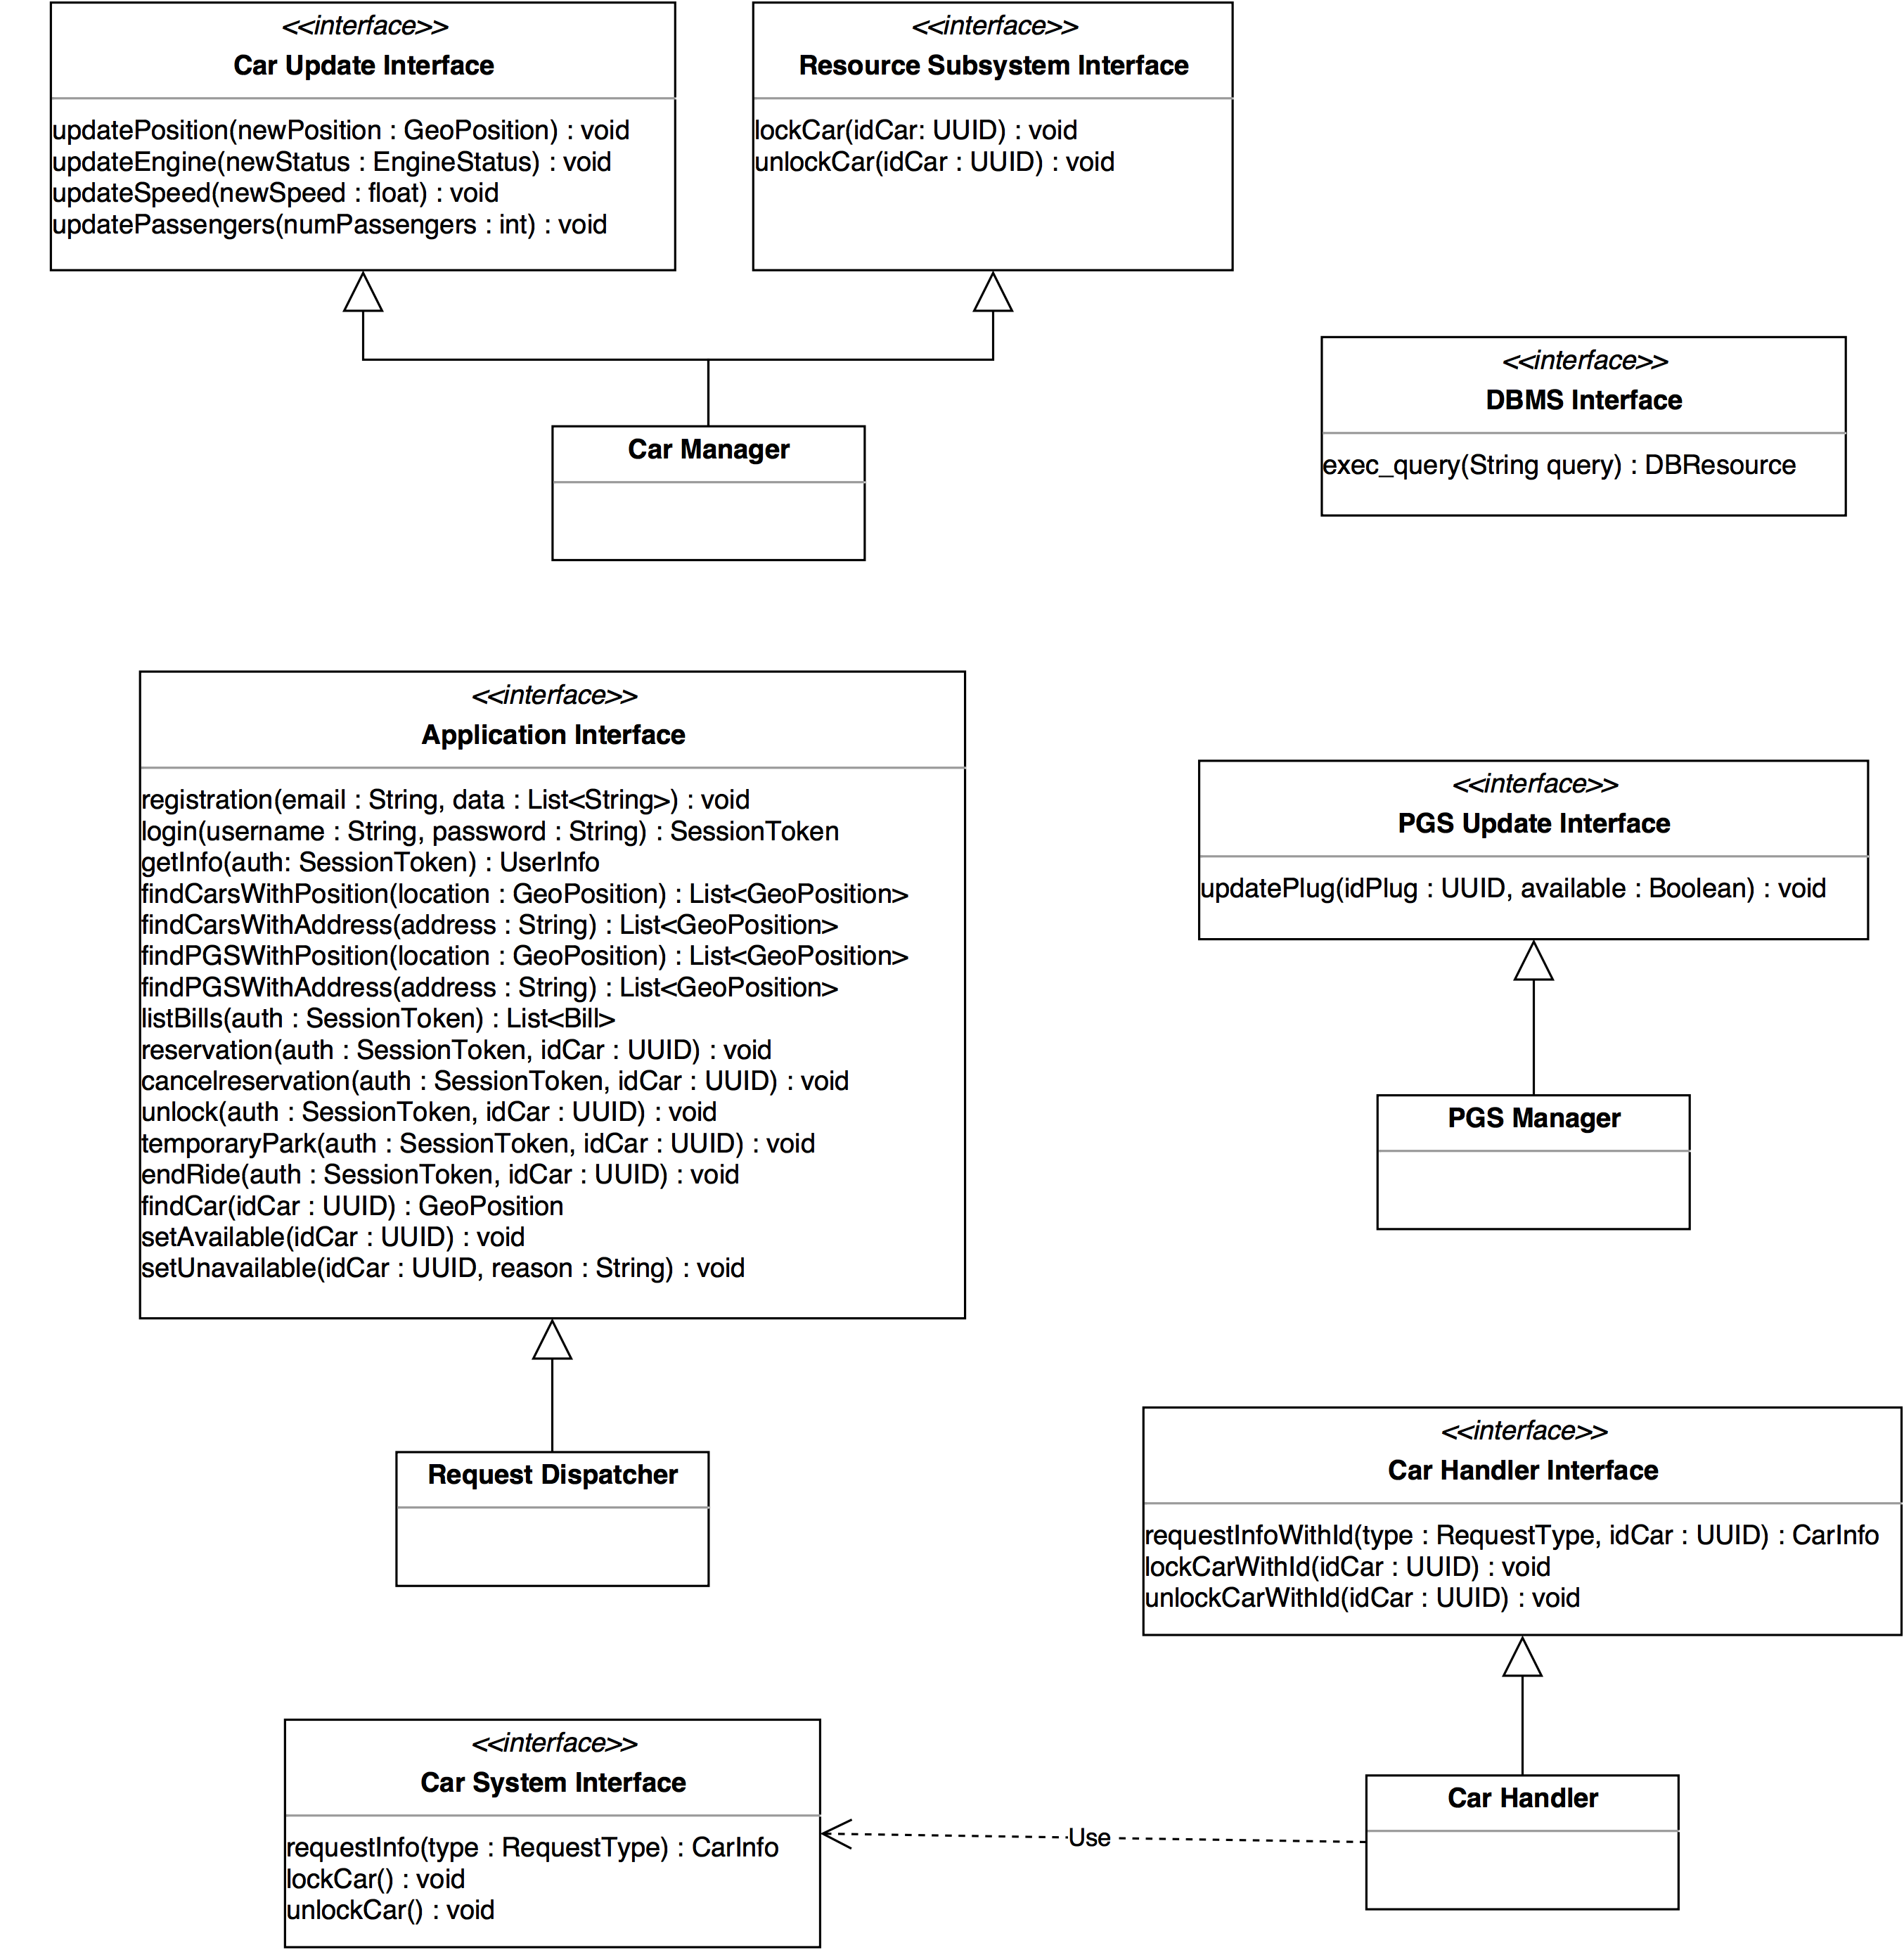
\includegraphics[width=430pt]{component_interfaces.png}
	}
	\caption{Component Interfaces}
	\label{compinterfaces}
\end{figure}

\subsection{Selected Architectural Styles and Patterns}

% Architecture Overall?
diviso in tre tier?

\subsubsection{Protocols}

cos'è REST
usiamo RESTful APIs (cioè stateless web interfaces)
stateless tranne per gli authentication token (OAuth passed via Authentication header)
quasi tutti necessitano di autenticazione (segnare quali con (*) tipo)

endpoint diversi per diverse funzioni

risposta con oggetti in notazione JSON

risposta con stato HTTP:
- 200 OK richiesta con successo
- 400 Bad Request no successo, + campo error con descrizione errore
- 401 Authorization Required se il token non è corretto
- 500 Server Error per errori server side

\paragraph{Application}
no need to pass username and car id, this is inferred from the auth token


\begin{itemize}
	\item{Registration:}\\
	\begin{tabular}{ | l l }
		\textit{Description} & Sign up to PowerEnJoy with an email, a licence and personal data \\
		\textit{Endpoint} & \code{/registration} \\ 
		\textit{Verb} & POST \\  
		\textit{Parameters} & \code{email}, \code{licence\_id} or \code{licence\_photo}, \code{name}, \code{dob}, \code{address}, \code{payment\_method} \\
		\textit{Response} & \code{200 OK} if successful.		
	\end{tabular}
	
	\item{Login:}\\
	\begin{tabular}{ | l l }
		\textit{Description} & Login to the application \\
		\textit{Endpoint} & \code{/login} \\ 
		\textit{Verb} & POST \\  
		\textit{Parameters} & \code{username}, \code{password} \\
		\textit{Response} & \code{auth\_token}
	\end{tabular}
	
	\item{Get user Info:}\\
		\begin{tabular}{ | l l }
			\textit{Description} & Get information related to the current user\\
			\textit{Endpoint} & \code{/userinfo} \\ 
			\textit{Verb} & GET \\  
			\textit{Parameters} & \code{auth\_token} \\
			\textit{Response} & \code{username}, \code{email}, \code{licence\_id}, \code{date\_of\_birth},  \code{address}, \code{curr\_reservation}
		\end{tabular}
	
	\item{Update the user's data:}\\
	\begin{tabular}{ | l l }
		\textit{Description} & Update the user's personal data to new ones\\
		\textit{Endpoint} & \code{/userinfo} \\ 
		\textit{Verb} & PATCH \\  
		\textit{Parameters} & \code{auth\_token}, optional: \code{email}, \code{password}, \code{address}, \code{payment\_method}  \\
		\textit{Response} & \code{200 OK} if successful
	\end{tabular}

	\item{Find cars with position:}\\
	\begin{tabular}{ | l l }
		\textit{Description} & Lists available cars close to the specified position\\
		\textit{Endpoint} & \code{/findcars/position/\{lat\}/\{long\}} \\ 
		\textit{Verb} & GET \\  
		\textit{Parameters} & None \\
		\textit{Response} & Set of \code{(car\_id, lat, long, battery)}
	\end{tabular}
	
	\item{Find cars with address:}\\
	\begin{tabular}{ | l l }
		\textit{Description} & Lists available cars close to the specified address\\
		\textit{Endpoint} & \code{/findcars/address/\{address\}} \\ 
		\textit{Verb} & GET \\  
		\textit{Parameters} & None \\
		\textit{Response} & Set of \code{(car\_id, lat, long, battery)}
	\end{tabular}
	
	\item{Find safe areas with position:}\\
	\begin{tabular}{ | l l }
		\textit{Description} & Lists safe areas close to the specified position\\
		\textit{Endpoint} & \code{/findsafeareas/position/\{lat\}/\{long\}} \\ 
		\textit{Verb} & GET \\  
		\textit{Parameters} & None \\
		\textit{Response} & Set of \code{(lat, long)}
	\end{tabular}

	\item{Find safe areas with address:}\\
	\begin{tabular}{ | l l }
		\textit{Description} & Lists safe areas close to the specified address\\
		\textit{Endpoint} & \code{/findsafeareas/address/\{address\}} \\ 
		\textit{Verb} & GET \\  
		\textit{Parameters} & None \\
		\textit{Response} & Set of \code{(lat, long)}
	\end{tabular}
	
	\item{Find power grid stations with position:}\\
	\begin{tabular}{ | l l }
		\textit{Description} & Lists power grid stations close to the specified position\\
		\textit{Endpoint} & \code{/findstations/position/\{lat\}/\{long\}} \\ 
		\textit{Verb} & GET \\  
		\textit{Parameters} & None \\
		\textit{Response} & Set of \code{(lat, long)}
	\end{tabular}

	\item{Find safe areas with address:}\\
	\begin{tabular}{ | l l }
		\textit{Description} & Lists safe areas close to the specified address\\
		\textit{Endpoint} & \code{/findstations/address/\{address\}} \\ 
		\textit{Verb} & GET \\  
		\textit{Parameters} & None \\
		\textit{Response} & Set of \code{(lat, long)}
	\end{tabular}
	
	\item{Make a reservation:}\\
	\begin{tabular}{ | l l }
		\textit{Description} & Creates a new reservation for a car\\
		\textit{Endpoint} & \code{/reservation} \\ 
		\textit{Verb} & POST \\  
		\textit{Parameters} & \code{auth\_token}, \code{carId} \\
		\textit{Response} & \code{200 OK} if successful
	\end{tabular}
	
	\item{Cancel a reservation:}\\
	\begin{tabular}{ | l l }
		\textit{Description} & Cancels the user's current reservation if there's one\\
		\textit{Endpoint} & \code{/reservation} \\ 
		\textit{Verb} & DELETE \\  
		\textit{Parameters} & \code{auth\_token}  \\
		\textit{Response} & \code{200 OK} if successful
	\end{tabular}
	
	\item{Unlock a car:}\\
	\begin{tabular}{ | l l }
		\textit{Description} & Unlocks the car that is currently reserved\\
		\textit{Endpoint} & \code{/unlock} \\ 
		\textit{Verb} & POST \\  
		\textit{Parameters} & \code{auth\_token}, \code{unlock\_id}  \\
		\textit{Response} & \code{200 OK} if successful
	\end{tabular}
	
	\item{Temporary parking:}\\
	\begin{tabular}{ | l l }
		\textit{Description} & Puts the car in temporary parking\\
		\textit{Endpoint} & \code{/parking} \\ 
		\textit{Verb} & POST \\  
		\textit{Parameters} & \code{auth\_token}  \\
		\textit{Response} & \code{200 OK} if successful
	\end{tabular}
	
	\item{End ride:}\\
	\begin{tabular}{ | l l }
		\textit{Description} & Concludes the current ride\\
		\textit{Endpoint} & \code{/endride} \\ 
		\textit{Verb} & POST \\  
		\textit{Parameters} & \code{auth\_token}  \\
		\textit{Response} & \code{200 OK} if successful
	\end{tabular}
	
	\item{List bills:}\\
	\begin{tabular}{ | l l }
		\textit{Description} & Shows all the user's bills\\
		\textit{Endpoint} & \code{/bills} \\ 
		\textit{Verb} & GET \\  
		\textit{Parameters} & \code{auth\_token}  \\
		\textit{Response} & Set of \code{(bill\_id, date, amount, payment\_status)}
	\end{tabular}
	
	\item{Pay bill:}\\
	\begin{tabular}{ | l l }
		\textit{Description} & Triggers a transaction to pay an outstanding bill if the user has one\\
		\textit{Endpoint} & \code{/paybill} \\ 
		\textit{Verb} & POST \\  
		\textit{Parameters} & \code{auth\_token}, \code{bill\_id}  \\
		\textit{Response} & \code{200 OK} if successful
	\end{tabular}

\end{itemize}


\paragraph{Maintenance}

\begin{itemize}
	\item{Find cars needing maintenance:}\\
	\begin{tabular}{ | l l }
		\textit{Description} & Lists all the cars in the systems with problems to solve\\
		\textit{Endpoint} & \code{/maintenancelist} \\ 
		\textit{Verb} & GET \\  
		\textit{Parameters} & \code{maintenance\_key}  \\
		\textit{Response} & Set of \code{(car\_id, lat, long, description)}
	\end{tabular}
	
	\item{Set car as available:}\\
	\begin{tabular}{ | l l }
		\textit{Description} & Sets a car as available\\
		\textit{Endpoint} & \code{/setcar/\{car\_id\}} \\ 
		\textit{Verb} & PUT \\  
		\textit{Parameters} & \code{maintenance\_key}, \code{availability}  \\
		\textit{Response} & \code{200 OK} if successful
	\end{tabular}
	
	\item{Set car as unavailable:}\\
	\begin{tabular}{ | l l }
		\textit{Description} & Sets a car as unavailable\\
		\textit{Endpoint} & \code{/setcar/\{car\_id\}} \\ 
		\textit{Verb} & PUT \\  
		\textit{Parameters} & \code{maintenance\_key}, \code{availability}, \code{description}  \\
		\textit{Response} & \code{200 OK} if successful
	\end{tabular}
\end{itemize}

autenticazione con chiave di accesso
basic http authentication

\paragraph{Sensors}

\begin{itemize}
	\item{Update from car:}\\
	\begin{tabular}{ | l l }
		\textit{Description} & Submits updates about the car to the server\\
		\textit{Endpoint} & \code{/updatecar} \\ 
		\textit{Verb} & POST \\  
		\textit{Parameters} & \code{car\_key}, \code{lat}, \code{long}, \code{speed}, \code{direction}, \code{engine\_status}, \code{lock\_status}, \code{passengers}\\
		\textit{Response} & \code{200 OK} if successful
	\end{tabular}
	
	\item{Update from power grid station:}\\
	\begin{tabular}{ | l l }
		\textit{Description} & Submits updates about the plugs in the station to the server\\
		\textit{Endpoint} & \code{/updateplug} \\ 
		\textit{Verb} & POST \\  
		\textit{Parameters} & \code{pgs\_key}, \code{plugs} (set of \code{(plug\_id, availability)})\\
		\textit{Response} & \code{200 OK} if successful
	\end{tabular}

\end{itemize}

a unique key for every car and station


tutte le richieste sono protette da TLS. full stop.

i comandi alle macchine vengono mandati aprendo un socket sul sistema della macchina e inviando comandi

\subsubsection{Patterns}
% mvc
% facade
% client-server
% event-driven architecture
% adapter?

\subsection{Other Design Decisions}

\newpage

\section{Algorithm Design}

\paragraph{}
In this section we are going to present potential algorithms to use when implementing the application.

We analyze two different functionalities that we want to implement:
\begin{itemize}
	\item{Calculating the discount to apply to a bill at the end of a ride;}
	\item{Finding and choosing a charging station to propose to the user when the Money Saving Option is activated.}
\end{itemize}

\paragraph{}
We decided to use Java-like pseudo-code as it is clear and easy to understand, and at the same time a language that we feel comfortable using.

\subsection{Discount calculation}

\lstinputlisting{Discounts.java}

\paragraph{}
We sum the individual discounts before applying them, to avoid one discount lessening the effects of others like it would happen if we applied them in sequence. This makes it so every discount is always worth the same and users aren't penalized for obtaining more than one discount at a time.

\paragraph{}
NB: the discount can vary from a maximum of 70\% to a minimum of -30\% (a 30\% overcharge).

\paragraph{}
The time complexity of this algorithm is $\theta(n)$, where $n$ is the number of power grid stations saved in the system, because we need to cycle through every station to find the distance from the car to the closest station.

This is not necessarily the best solution. For example this could be improved by subdividing the stations in zones so that we can check only the ones in which the car is currently located.

\newpage
\subsection{Finding a station for the Money Saving Option}

	\lstinputlisting{MoneySavingOption.java}

\paragraph{}
Because of our requirements this algorithm must take in account the distribution of cars and make it as uniform as possible.

To realize this, our algorithm:
\begin{itemize}
	\item{takes the user's final destination as input;}
	\item{looks for all the power grid stations reasonably close to the destination;}
	\item{chooses among all the acceptable stations the one that would make distribution more balanced (the one with the least cars nearby).}
\end{itemize}

\paragraph{}
The time complexity of this algorithm is $\theta(n) + \theta(m \cdot c) + \theta(m)$ or $\theta(n + m (1+c))$, where $n$ is the number of charging stations in the system, $m$ the number of acceptable stations, and $c$ the number of cars close to them.

This can also be improved by subdividing the stations in zones.
Another option could be saving the number of cars near every station in advance, and updating it every time a car is parked nearby or driven away, without having to recompute the value every time it is needed.

\newpage

\section{User Interface Design}

\subsection{Mockups}
% rimandare al RASD

\subsection{UX Diagrams}

\subsection{BCE Diagrams}

\newpage

\section{Requirements Traceability}
To make sure that every component of our architecture is actually needed, we now show which components are used to fulfill each goal that we identified in the Requirement Analysis and Specification Document.

\begin{description}
	\item[{[G1]}]{Guests must be able to register as users by choosing a username and providing their personal data, driving license and payment information. They will receive a password at the email address they specified.}
	\begin{itemize}
		\item{Application Subsystem}
		\item{Request Dispatcher}
		\item{Registration Component}
		\item{Signup API}
		\item{Driving Licence API}
		\item{Model}
		\item{DBMS}
	\end{itemize}
	\item[{[G2]}]{Users must be able to login with the username/email inserted and the password received on registration.}
	\begin{itemize}
		\item{Application Subsystem}
		\item{Request Dispatcher}
		\item{Login Component}
		\item{Model}
		\item{DBMS}
	\end{itemize}
	\item[{[G3a]}]{Users must be able to find the location and battery charge of all the available cars within a certain distance from their current location.}
	\begin{itemize}
		\item{Application Subsystem}
		\item{Request Dispatcher}
		\item{Car Search Component}
		\item{Maps API}
		\item{Model}
		\item{DBMS}
	\end{itemize}
	\item[{[G3b]}]{Users must be able to find the location and battery charge of all available cars around a specified location.}
	\begin{itemize}
		\item{Application Subsystem}
		\item{Request Dispatcher}
		\item{Car Search Component}
		\item{Maps API}
		\item{Model}
		\item{DBMS}
	\end{itemize}
	\item[{[G4]}]{Users must be able to reserve a car for up to one hour before they pick it up. If they don't take the car before the time expires they are charged a fixed fee of 1 EUR.}
	\begin{itemize}
		\item{Application Subsystem}
		\item{Request Dispatcher}
		\item{Reservation Manager}
		\item{Payment Component}
		\item{Model}
		\item{DBMS}
	\end{itemize}
	\item[{[G5]}]{Users must be able to cancel a reservation if they decide to not actually use the car.}
	\begin{itemize}
		\item{Application Subsystem}
		\item{Request Dispatcher}
		\item{Reservation Manager}
		\item{Model}
		\item{DBMS}
	\end{itemize}
	\item[{[G6]}]{A user that reaches a car reserved by them must have a way to tell the system they’re nearby, so that the system unlocks the car and the user may enter.}
	\begin{itemize}
		\item{Application Subsystem}
		\item{Request Dispatcher}
		\item{Unlocking Component}
		\item{Resource Management Subsystem}
		\item{Car Manager}
		\item{Car Handler}
		\item{Car Internal System}
		\item{Model}
		\item{DBMS}
	\end{itemize}
	\item[{[G7]}]{The system must charge the user who reserved the car from the moment the engine is ignited after unlocking it. The user is charged for a given	amount of money per minute.}
	\begin{itemize}
		\item{Car Internal System}
		\item{Resource Management Subsystem}
		\item{Car Manager}
		\item{DBMS}
	\end{itemize}
	\item[{[G8]}]{The system must allow the user to see the amount they’re being charged through a screen on the car.}
	\begin{itemize}
		\item{Car Application}
		\item{Application Subsystem}
		\item{Request Dispatcher}
		\item{Ride Manager}
		\item{Model}
		\item{DBMS}
	\end{itemize}
	\item[{[G9]}]{The system must stop charging the user as soon as the car is parked in a safe area and the user exits the car notifying the system that they ended their ride.}
	\begin{itemize}
		\item{Car Internal System}
		\item{Resource Management Subsystem}
		\item{Car Manager}
		\item{Application Subsystem}
		\item{Request Dispatcher}
		\item{Ride Manager}
		\item{Payment}
		\item{Payment API}
		\item{Model}
		\item{DBMS}
	\end{itemize}
	\item[{[G10]}]{Users must be able to leave a car without losing the reservation by informing the system that they’re only temporarily parking; in this case the system continues on charging the user. The user should be able to end the ride without coming back to the car if they so choose.}
	\begin{itemize}
		\item{Application Subsystem}
		\item{Request Dispatcher}
		\item{Parking Component}
		\item{Model}
		\item{DBMS}
	\end{itemize}
	\item[{[G11]}]{The system must lock the car automatically after the user exits the car.}
	\begin{itemize}
		\item{Resource Management Subsystem}
		\item{Car Manager}
		\item{Car Handler}
		\item{Car Internal System}
	\end{itemize}
	\item[{[G12]}]{The system must provide a money saving option to the user, proposing a suitable power grid station near the user’s final destination. The user will get a discount if they park the car there and plug it in the power grid.}
	\begin{itemize}
		\item{Application Subsystem}
		\item{Request Dispatcher}
		\item{PGS Search Component}
		\item{Maps API}
		\item{DBMS}
		\item{PGS Internal System}
		\item{PGS Manager}
	\end{itemize}
	\item[{[G13]}]{The stations proposed by the system with the money saving option must be chosen in a way that ensures a uniform distribution of cars in the city.}
	\begin{itemize}
		\item{(None)}
	\end{itemize}
	\item[{[G14]}]{The system must apply a discount of 10\% on the last ride if the user took at least two other passengers onto the car.}
	\begin{itemize}
		\item{Car Internal System}
		\item{Resource Management Subsystem}
		\item{Car Manager}
		\item{Model}
		\item{DBMS}
		\item{Application Subsystem}
		\item{Ride Manager}
		\item{Payment Component}
	\end{itemize}
	\item[{[G15]}]{The system must apply a discount of 20\% on the last ride if the car is left with more than 50\% of remaining battery charge.}
	\begin{itemize}
		\item{Car Internal System}
		\item{Resource Management Subsystem}
		\item{Car Manager}
		\item{Application Subsystem}
		\item{Ride Manager}
		\item{Payment Component}
		\item{Model}
		\item{DBMS}
	\end{itemize}
	\item[{[G16]}]{The system must apply a discount of 30\% on the last ride if the car is left at special parking areas where they can be recharged, and the user takes care of plugging the car into the power grid.}
	\begin{itemize}
		\item{Car Internal System}
		\item{Resource Management Subsystem}
		\item{Car Manager}
		\item{Application Subsystem}
		\item{Request Dispatcher}
		\item{Ride Manager}
		\item{Payment Component}
		\item{PGS Internal System}
		\item{PGS Manager}
		\item{Model}
		\item{DBMS}
	\end{itemize}
	\item[{[G17]}]{The system must charge 30\% more if the car is left at more than 3 km from the nearest power grid station or with less than 20\% remaining battery charge.}
	\begin{itemize}
		\item{Car Internal System}
		\item{Resource Management Subsystem}
		\item{Car Manager}
		\item{Application Subsystem}
		\item{Request Dispatcher}
		\item{Ride Manager}
		\item{Payment Component}
		\item{Maps API}
		\item{Model}
		\item{DBMS}
	\end{itemize}
	\item[{[G18]}]{Users with outstanding bills cannot have access to the cars and reservations until the bills are paid.}
	\begin{itemize}
		\item{Application Subsystem}
		\item{Request Dispatcher}
		\item{Reservation Manager}
		\item{Model}
		\item{DBMS}
	\end{itemize}
	\item[{[G19]}]{Users with outstanding bills should have a way to pay them.}
	\begin{itemize}
		\item{Application Subsystem}
		\item{Request Dispatcher}
		\item{Payment}
		\item{Model}
		\item{DBMS}
	\end{itemize}
	\item[{[G20]}]{Available cars should actually be available to the user and in good conditions (i.e. not dirty, damaged, and/or with low battery).}
	\begin{itemize}
		\item{Application Subsystem}
		\item{Request Dispatcher}
		\item{Report Manager}
		\item{Resource Management Subsystem}
		\item{Car Manager}
		\item{Model}
		\item{DBMS}
	\end{itemize}
	\item[{[G21]}]{Users must be able to easily find power grid stations.}
	\begin{itemize}
		\item{Application Subsystem}
		\item{Request Dispatcher}
		\item{PGS Search Component}
		\item{Model}
		\item{DBMS}
	\end{itemize}
	
\end{description}

Every component in our architecture is used by at least one goal.

\newpage

\section{Effort Spent}

\section{Revisions}

\subsection{Changelog}
\begin{itemize}
	\item{DD v1.0, published on December 11, 2016}
\end{itemize}
\end{document}
